\chapter{Theorie}


\section{Der Plasmazustand}

Die üblichen drei Aggregatszustände sind nach der Energie und \glqq{}Freiheit\grqq{} der Teilchen geordnet. Führt man zum Beispiel Energie einem Festkörper zu, brechen die festen Bindungen zwischen den einzelnen Atomen oder Molekülen, die die Struktur des Festkörpers erhalten, und die Teilchen sind nur noch schwach aneinander gebunden. Die Substanz ist nun flüssig. Gibt man dieser Flüssigkeit noch mehr Energie zu, lösen sich auch die schwächeren Verbindungen. Die Teilchen sind dann völlig unabhängig voneinander und bilden ein Gas. Führt man dem Gas noch weitere Energie zu, lösen sich die äußersten Elektronen teilweise von ihren Atomrümpfen und es bildet sich ein \textit{Plasma}. 

Die Bezeichnung \glqq{}Plasma\grqq{} wurde 1928 von Irving Langmuir eingeführt, den der Transport der freien Ladungsträger in der Entladung an den Transport von roten und weißen Blutkörperchen im Blutplasma erinnerte \cite{langmuirOscillationsIonizedGases1928,hirshGaseousElectronics2012}.

\subsection{Allgemeine Eigenschaften eines Plasmas}

Zur Beschreibung von Gasen ist es ausreichend, nur die lokalen Stöße zwischen den Teilchen zu betrachten, wie es in der kinetischen Gastheorie geschieht \cite{feynmanrichardpFeynmanLecturesPhysics1964}. Bei einem Plasma ist es dagegen nicht möglich, neutrale Teilchen, Atomrümpfe und Elektronen als separate, herkömmliche Gase zu beschreiben. Der hauptsächliche Unterschied zwischen Gas und Plasma liegt im kollektiven Verhalten \cite{pielPlasmaPhysicsIntroduction2010}. Während die Van-der-Waals-Wechselwirkungen zwischen Gasmolekülen mit $ r^{-6} $ so schnell abklingen, dass die Stoßbeschreibung ausreicht, wirkt die elektrische Kraft, die mit $ r^{-2} $ abklingt, als Fernwirkung zwischen Teilchen an verschiedenen Orten. Die Dominanz dieser elektrischen Wirkungen über die Stöße zwischen den Teilchen unterscheidet Gas und Plasma.

\subsubsection{Quasineutralität und Abschirmung}

Das Plasma als Ganzes ist elektrisch neutral, obwohl positive und negative Ladungsträger im Plasma frei voneinander vorhanden sind. Betrachtet man also ein hinreichend großes Volumen innerhalb des Plasmas, ist die Anzahl positiver und negativer Ladungsträger in etwa gleich.\footnote{Bzw. gewichtet mit den Ladungen der Ladungsträger im Falle mehrfacher Ionisation.} Dies ist durch die elektrischen Fernwirkungen im Plasma bedingt. Befänden sich beispielsweise in einer Gegend mehr positive als negative Ladungen, würden positive Ladungen von der Ladung abgestoßen und negative Ladungen angezogen. Es stellt sich ein Ausgleich der Raumladung ein.

Die Größenordnung, ab der ein Plasmavolumen groß genug ist, um Quasineutralität zu zeigen, wird durch die \textit{Debyelänge} gegeben. Wird eine äußere Ladung ins Plasma eingebracht, zieht diese ungleichnamige Ladungen aus dem Plasma an. Um die eingebrachte Ladung bildet sich dann eine Raumladungszone entgegengesetzter Ladung, die das Feld abschirmt. Diese Abschirmung geschieht exponentiell mit der Debyelänge $\lambda_{De,Di}$ als Skalenfaktor. Diese ist für Elektronen und Ionen (jeweils durch $ e $ bzw. $ i $ im Index gekennzeichnet) separat zu berechnen, da diese unterschiedliche Temperaturen $ T_{e,i} $ haben können. Dabei gilt \cite{pielPlasmaPhysicsIntroduction2010}
\begin{align*}
	\lambda_{De,Di}  = \sqrt{\dfrac{\epsilon_0k_BT_{e,i}}{n_{e,i}e_0^2}},
\end{align*}
wobei $ \epsilon_0 $ die elektrische Feldkonstante, $ k_B $ die Boltzmannkonstante, $ n_{e,i} $ die entsprechende Dichte und $ e_0 $ die Elementarladung bezeichnen.
Zusammenfassend kann man dann die sogenannte linearisierte Debyelänge $ \frac{1}{\lambda_D^2} = \frac{1}{\lambda_{De}^2} + \frac{1}{\lambda_{Di}^2} $ bilden. Um ein Plasma mit Quasineutralität zu gewährleisten, müssen sich in einer Kugel mit der Debyelänge als Radius viele Teilchen befinden \cite{pielPlasmaPhysicsIntroduction2010}: $ n\cdot\lambda_{D}^{3}\gg 1 $

\subsubsection{Zeitskala der elektrischen Wirkungen}

Der Ausgleich von Raumladungszonen im Plasma geschieht wegen des Impulses der Elektronen durch Einschwingen. Die Elektronen können also als Ensemble Schwingungen vollführen, welche die \textit{Plasmafrequenz} $ \omega_{P} $ haben. Eine analoge Plasmafrequenz lässt sich auch für die Ionen aufstellen \cite{pielPlasmaPhysicsIntroduction2010}:
\begin{align*}
	\omega_{Pe,Pi} = \sqrt{ \dfrac{n_{e,i} e_0^2}{\epsilon_0m_{e,i}}}
\end{align*}
Dabei ist $ m_{e,i} $ die Elektronen- bzw. Ionenmasse.
Eine zweite Zeitskala wird durch die Stoßfrequenz $ \nu $ gegeben, die beschreibt, wie häufig ein bestimmtes Teilchen mit anderen kollidiert. Die Dominanz der elektrischen Wirkungen über die normale Gaskinetik zeigt sich dann darin, dass die Plasmafrequenz in einem Plasma deutlich höher ist, als die Stoßfrequenz der Teilchen.

\subsubsection{Thermische und nicht-thermische Plasmen}

Die verschiedenen Spezies der Elektronen und Ionen sind in einem Plasma oft nicht im  thermodynamischen Gleichgewicht. Dies liegt daran, dass die Elektronen viel leichter sind als die Ionen und deshalb durch das elektrische Feld deutlich schneller und auf höhere Energien beschleunigt werden. Da beim Stoß eines leichten Elektrons mit einem schweren Ion jedoch nur sehr wenig Energie an das Ion übertragen wird, dauert eine Thermalisierung sehr lange. Die Ionen können, trotz der hohen Elektronentemperatur, als \glqq{}Teilgas\grqq{} deshalb deutlich kälter sein. Bei den in dieser Arbeit betrachteten Plasmen erhitzen sich die Elektroden zum Beispiel nur auf ca. 70-80\Grad C, was eine ähnlich niedrige Ionen- und Neutralgastemperatur impliziert.

Während die in dieser Arbeit betrachtete Glimmentladung damit ein nicht-thermisches Plasma ist, gibt es auch thermische Plasmen wie z.B. Lichtbogenentladungen, bei denen Elektronen- und Ionentemperatur im Gleichgewicht sind \cite{keudellVorlesungsskriptEinfuhrungPlasmaphysik2008}.



\subsection{Das Paschen-Gesetz und der Zündprozess}

Das Paschen-Gesetz beschreibt die Zündspannung eines Plasmas abhängig von Druck $ p $ und vom Abstand der Elektroden $ d $:
\begin{align*}
	U = B \cdot \dfrac{pd}{C + \ln pd}
\end{align*}
Dabei sind $ A $  und $ B $ gasspezifische Konstanten, $ C = \ln\frac{A}{\ln(1+1/\gamma_I)} $ und $ \gamma_I $ — die Anzahl der Sekundärelektronen, die ein Ion auf der Kathode im Durchschnitt direkt herauslöst — eine Materialkonstante.  

Dass die Zündspannung nach dem Paschen-Gesetz nur vom Produkt $ p\cdot d $ abhängt, liegt am Mechanismus des Durchbruchs.
Während der Zündung werden freie Elektronen von der angelegten Spannung beschleunigt, welche dann Atome ionisieren können und so durch die Produktion weiterer Elektronen eine Elektronenlawine erzeugen. Diese führt schließlich zur Ausbildung eines Plasmakanals. Dafür ist es wichtig, dass ein Elektron auf dem Weg zwischen zwei Stößen so sehr beschleunigt wird, dass es beim nächsten Stoß wieder ein Atom ionisieren kann. Da bei einem höheren Druck die freie Weglänge der Elektronen zwischen den Atomen kleiner ist, ist die erreichte Energie proportional zu $ 1/p $. Gleichzeitig ist die beschleunigende Feldstärke bei gegebener Spannung an den Elektroden proportional zu $ 1/d $. Insgesamt ist also die erreichte Energie und damit auch die nötige Zündspannung eine Funktion des Produkts $ pd $.

\begin{figure}[H]
	\centering
	\includesvg[width=0.85\linewidth]{plots/paschen_kurve}
	\caption{Die Paschenkurven von Helium, Argon und Luft bei \qty{1e5}{\pascal}. Die theoretischen Zündspannungen bei der Elektrodenentfernung von \qty{100}{\um} sind angeschrieben. (Konstanten A = \qty{2,25}{Pa^{-1}.m^{-1}}  ,B = \qty{25,5}{V.Pa^{-1}.m^{-1}} und $ \gamma =$ \num{0,1} aus \cite{lehrElectricalBreakdownGases2017,bohmRetardingfieldAnalyzerMeasurements1993}.)}
	\label{fig:paschen_kurve}
\end{figure}

Wie in Abb. \ref{fig:paschen_kurve} erkennbar, steigt für große $ pd $ die nötige Zündspannung an, zum Beispiel, wenn der Elektrodenabstand sehr groß wird. Bei kleineren $ pd $ erreicht diese sogenannte \textit{Paschen-Kurve} zunächst ein Minimum und steigt dann für noch kleinere $ pd $ stark an. Da bei hohen Zündspannungen viel Strom fließt und einen Lichtbogen erzeugt, ist es für Glimmentladungen in Helium als Arbeitsgas notwendig, möglichst nah am Minimum der Paschen-Kurve zu arbeiten. Dieses tritt bei einem konstanten $ pd $-Produkt auf  \cite{paschenUeberFunkenuebergangLuft1889,rajzerGasDischargePhysics1997}.

Um die minimale Zündspannung zu ermöglichen, muss deshalb der Abstand der Elektroden bei höherem Druck stark verringert werden. In dieser Arbeit werden die Elektroden \qty{100}{\um} voneinander entfernt gehalten. Damit ist der Abstand noch deutlich über dem Paschenminimum von etwa \qty{30}{\um} oder sogar \qty{6}{\um} bei Argon (siehe Abb. \ref{fig:paschen_kurve}). Dies ist in der Praxis aber üblich, da sehr kleine Elektrodenentfernungen nur schwer zu realisieren sind \cite{bruggemanFoundationsAtmosphericPressure2017}.

\subsection{Mikroplasmen}

Plasmen, die auf einer Skala von \qty{1}{\um} bis \qty{1}{\mm} betrieben werden, werden als Mikroplasmen bezeichnet \cite{edenMicrocavityPlasmaDevices2005}. Um bei so kleinen Elektrodenabständen ein Plasma zu zünden, werden Drücke in der Größenordnung des Atmosphärendrucks von etwa \qty{1e5}{\Pa} benötigt. In Abbildung \ref{fig:paschen_kurve} ist gut erkennbar, dass das Paschen-Minimum bei Atmosphärendruck in diese Größenordnung des Elektrodenabstandes fällt. Zusätzlich zum Betrieb bei oder sogar über Atmosphärendruck haben Mikroplasmen noch viele weitere interessante Eigenschaften, welche sich teilweise in dieser Arbeit beobachten lassen. Besonders die hohe Leistungsdichte, die sich in solchen Plasmen ergibt, lässt sich in einer größeren Entladung nur schwer erreichen. Beispielsweise wird die Leistungsdichte des hier betrachteten Mikroplasma auf \qty{3e4}{W.cm^{-3}} geschätzt.\\

Der Betrieb von Mikroplasmen ist in vielen verschiedenen Elektrodengeometrien möglich. So können zum Beispiel Hohlräume der entsprechenden Größenordnung auf der Kathode verwendet werden \cite{dzikowskiElectricFieldStrengths2022}. Auch das flächige Plasma einer dielektrisch behinderten Oberflächenentladung (SDBD) ist aus einzelnen Mikroplasmen aufgebaut \cite{hoderComplexInteractionSubsequent2017}. Die wohl einfachste Elektrodengeometrie mit der ein Mikroplasma gezündet werden kann, sind zwei parallele, ebene Elektroden. Anders als z.B. bei dielektrisch behinderten Entladungen kann ein Plasma so mit Gleichstrom betrieben werden. Deshalb und aufgrund der Einfachheit des Aufbaus wird in dieser Arbeit eine solche Entladung untersucht.

\section{Passive Thermosonden}
Die passive Thermosonde (PTP) und ihr Messprinzip gehen auf eine Arbeit von Thornton \cite{thorntonSubstrateHeatingCylindrical1978} im Jahre 1978 zurück. 
Passive Thermosonden ermöglichen die Messung von Energieströmen im Plasma, indem sie die Erwärmung eines Testkörpers messen. Da diese Sonden einfach zu verstehen und bauen sind, werden sie in der Plasmaphysik häufig zur Diagnostik benutzt \cite{benediktFoundationsMeasurementElectrons2021,gauterCalorimetricProbeMeasurements2017,rosenfeldtUsePassiveThermal2021a}.
Die Heizleistung ergibt sich als Bilanz vieler einzelner Energieströme auf die Sonde, zum Beispiel der Heizung durch Ladungsträger, Neutralteilchen und Strahlung, abgeführte Energie durch Sekundärelektronenemission und der Energiebilanz von Rekombinationsprozessen auf der Sondenoberfläche. 
%In Kombination mit anderen diagnostischen Verfahren kann der gesamte Energiestrom dann in die Komponenten aufgeschlüsselt werden.

\subsection{Aufbau der Sonde}
Der Sondenkopf besteht aus einem Dummy-Plättchen, das die Leistung des Plasmas aufnimmt. An dieses Plättchen sind durch Punktschweißen ein Typ-K Thermoelement und ein Kupferdraht befestigt \cite{haaseDynamicDeterminationSecondary2018}. Zur thermischen Isolierung des Plättchens steht dieses frei und ist nur über die Drähte befestigt \cite{kewitzInvestigationCommercialAtmospheric2015,cipoDiagnosticsProcessPlasma2020}. Über das Thermoelement kann der Temperaturverlauf des Sondenplättchens aufgezeichnet werden. Der Kupferdraht dient als elektrische Verbindung, die hier zum Zünden des Plasmas genutzt wird. Durchmesser und Dicke des Plättchens sind vom jeweiligen Aufbau abhängig. Je nach Größe und Leistung des Plasmas kann ein passender Durchmesser genutzt werden. Da in dieser Arbeit an einem Mikroplasma mit geringer Leistung gemessen wird, werden 5mm große Plättchen genutzt. Um eine empfindlichere Messung bei geringen Energieströmen zu erreichen, wird die Wärmekapazität des Plättchens mit einer Dicke von \qty{100}{\um} klein gehalten.
%?????

\subsection{Messprinzip}\label{messprinzip}

Die Energiebilanz des Substrats wird durch dessen Enthalpie $ H $ und deren Änderung $ \dot{H} $ beschrieben. Dabei ist $ \dot{H} $ die Bilanz der Leistung $ P_\text{in} $ an das und $ P_\text{out} $ von dem Substrat, vorausgesetzt es gibt keine Prozesse innerhalb des Plättchens. Über die Wärmekapazität $ C $ des Substrats ist die Änderung der Enthalpie mit der der Temperatur verbunden \cite{gauterCalorimetricInvestigationPlasma2018}
\begin{align*}
\dot{	H} = C \dot{T} = P_\text{in} - P_\text{out}.
\end{align*}
Wird das Plasma angeschaltet, heizt dieses das Plättchen. Gleichzeitig gibt es durch verschiedene Mechanismen eine  Abfuhr von Wärme aus dem Substrat, die unter $ P_\text{out} $ zusammengefasst wird. Wird nun das Plasma ausgeschaltet, fällt der heizende Wärmestrom weg und das Plättchen kühlt ab. Die Änderung der Enthalpie können wir mit zwei Gleichungen beschreiben \cite{gauterCalorimetricInvestigationPlasma2018}:
\begin{align*}
	\text{Heizen:}\quad \dot{H}_h &= C \dot{T}_h = P_\text{in} - P_{\text{out},h}\\
	\text{Kühlen:}\quad \dot{H}_c &= C \dot{T}_c =- P_{\text{out},c}
\end{align*}

Unter der Annahme, dass die abgeführte Leistung $ P_\text{out} $ nur von der Temperatur abhängig ist und nicht davon, ob das Plasma an- oder ausgeschaltet ist, kann $ P_\text{in} $ durch Vergleich beider Temperaturänderungen bestimmt werden \cite{thorntonSubstrateHeatingCylindrical1978}
\begin{align*}
	P_\text{in} = C( \dot{T}_h - \dot{T}_c).
\end{align*}

\subsection{Auswertungsmethodik}


Um eine Veränderung der Rahmenbedingungen während der Messung zu vermeiden, wird das Plasma dazu nur kurz (hier \qty{10}{\second}) angeschaltet, sodass zwischen den Messungen des Heizens und Abkühlens wenig Zeit vergeht und $ P_\text{out} $ als in beiden Fällen identisch angenommen werden kann. Die Messdaten sind dann Reihen solcher Aufheiz- und Abkühlphasen, die durch das Ein- und wieder Abschalten des Plasmas erzeugt werden. Im Temperaturverlauf der Sonde zeigen sich diese als Temperaturspitzen (siehe Abb. \ref{fig:peask_bsp}). Zur Auswertung der Daten wird hier die \textit{dT-Methode} \cite{rosenfeldtUsePassiveThermal2021,gauterCalorimetricInvestigationPlasma2018,hansenEnergyFluxMeasurements2019,hansenUnderstandingEnergyBalance2021} verwendet, die im Folgenden erklärt wird.\\

Bei konstanter Eingangsleistung kann man zeigen, dass die resultierende Temperaturkurve einem exponentiellen Verlauf folgt \cite{gauterCalorimetricInvestigationPlasma2018}:

\begin{align*}
	T_h(t) &= T_{eq} + \dfrac{P_\text{in}}{\alpha} - \left( \dfrac{P_\text{in}}{\alpha} \right) \exp\left( - \dfrac{\alpha}{C}t \right)\\
	T_c(t) &= T_{eq} + (T_{st} - T_{eq}) \exp\left( - \dfrac{\alpha}{C}t \right)
\end{align*}
Dabei ist $ T_{eq} $ die Gleichgewichtstemperatur, auf die das Plättchen ohne Plasma abkühlt, $ T_{st} $ die Temperatur am Anfang des Abkühlens und $ \alpha $ eine Konstante des Plättchens, die die Effizienz des Abkühlens beschreibt. Aufgrund des exponentiellen Charakters des Verlaufs, gibt es einen linearen Zusammenhang zwischen der Substrattemperatur und deren Ableitung.
\begin{align*}
 	\dfrac{\dd T_h}{\dd t} &= - \dfrac{\alpha}{C} \cdot T_h  + \dfrac{\alpha T_{eq} + P_\text{in}}{C}\\
 	\dfrac{\dd T_c}{\dd t} &= - \dfrac{\alpha}{C} \cdot T_c  + \dfrac{\alpha T_{eq}}{C}\\
\end{align*}

Dabei ist die Steigung für eine bestimmte Sonde konstant. Die Differenz der konstanten Terme ist dann proportional zur Heizleistung.
\begin{figure}[h]
	\centering
	\includesvg[width=\linewidth]{plots/peak_bsp}
	\caption{\textbf{a)} Beispielhafte Darstellung eines Temperaturpeaks. \textbf{b)} Der selbe Temperaturpeak in dT-Darstellung. Es werden lineare Fits an die linearen Bereiche gezeigt, deren Steigungen nahezu parallel sind.}
	\label{fig:peask_bsp}
\end{figure}

Trägt man wie in Abb. \ref{fig:peask_bsp} die Temperaturänderung gegen die Temperatur auf, erkennt man diese zwei linearen Bereiche, die dem Heiz- und Kühlprozess entsprechen. Beide zeigen die gleiche Steigung, die Heizkurve liegt jedoch in der Grafik oben. Durch lineare Regression lassen sich die beiden Kurven vergleichen. In der Theorie ergibt sich die Leistung einfach aus der Differenz der Achsenabschnitte multipliziert mit der Wärmekapazität der Sonde. Da die Steigungen in der Praxis jedoch fehlerbehaftet und nicht exakt gleich sind, wird die Differenz in der Mitte der Regressionsbereiche gebildet. Bei einer Differenzbildung der y-Achsenabschnitte hätte der Unterschied der Steigungen einen größeren Einfluss als nötig, da sich dieser außerhalb der Bereiche verstärkt.


\paragraph{Glättung der Datenreihe}
Um die Ableitung einer verrauschten Datenreihe zu bilden, ist es wichtig, die Daten vorher zu glätten, da die Differenzenbildung aufeinanderfolgender Werte das Rauschen in den Daten verstärkt. Dabei hat die Methode der Glättung einen großen Einfluss darauf, wie viel geglättet werden muss, um eine saubere Ableitung berechnen zu können. Dies liegt an den Eigenschaften der Faltung. Die Ableitung der Faltung einer Funktion mit einem Faltungskern ist gleich der Faltung der Funktion mit der Ableitung des Kerns \cite{forsythdavidComputerVisionModern2012}
\begin{align*}
	\dfrac{\dd }{\dd x} (f*k)(x) = f*\left(\!\dfrac{\dd k}{\dd x}\right).
\end{align*}
Eine einfache Glättung durch einen laufenden Mittelwert entspricht der Faltung mit einem rechteckigen Faltungskern der Länge $ l $ des Glättungsfensters. Damit entspricht die Ableitung der so geglätteten Funktion der Faltung mit einem Kern der Form
\begin{align*}
	\dfrac{\dd k}{\dd x} = \dfrac{1}{l} \left(\delta\left(x+ \dfrac{l}{2}\right) -\delta\left(x- \dfrac{l}{2}\right)\right).
\end{align*}
Die so berechnete Ableitung wäre also wieder nur die Differenz zweier einzelner Datenpunkte, die hier nur weiter auseinanderlägen.

Dieses Problem kann mit einer Methode aus dem Feld der automatischen Bildverarbeitung und -erkennung gelöst werden, da auch für die Kantenerkennung in Bildern die Ableitung von verrauschten Daten gebildet werden muss. Anstatt eines Rechteckfensters wird hier eine Gaußkurve zum Glätten verwendet \cite{forsythdavidComputerVisionModern2012,dengAdaptiveGaussianFilter1993}. Bei der Ableitung einer so geglätteten Kurve werden die Differenzen der Werte ganzer Bereiche gebildet, da die Ableitung der Gaußkurve nicht nur zwei Spitzen hat. Dies führt dazu, dass die so abgeleiteten Daten wesentlich weniger verrauscht sind, wie in Abb. \ref{fig:gaussglaettung} sichtbar wird. Zudem wird der Einfluss einzelner Ausreißer in den Daten verringert, sodass diese nicht zu abrupten Sprüngen in der Ableitung führen.
Um die Daten nicht übermäßig zu glätten, wird für die Gaußkurve hier eine Standardabweichung von 10 Datenpunkten, also $ \frac{1}{9} $ s, genutzt.

\begin{figure}[p]
\centering
\includesvg[width=0.96\linewidth]{plots/gaussglaettung}
\caption{Vergleich zwischen gaußartiger Glättung und laufendem Durchschnitt:\textbf{a)} Ungeglättete Datenreihe; \textbf{b,c)} Glättungskerne beider Art und deren Ableitungen. Beide Kerne haben die gleiche Standardabweichung. Die Ableitung des Gaußkerns ist zur besseren Sichtbarkeit vertikal vergrößert. In Grau: Ausschnitt aus dem Rohsignal als Beispiel; \textbf{d,e)} Mit den jeweiligen Kernen geglättetes Signal; \textbf{f,g)} Die Ableitungen der entsprechenden Signale; \textbf{h,i)} Die beider Art geglätteten Signale in dT-Darstellung.}
\label{fig:gaussglaettung}
\end{figure}

Beim Vergleich beider Methoden zeigt sich, dass ein Gaußkern zu einem deutlich rauschfreieren Ergebnis führt als eine Glättung mit einem Rechteckkern gleicher Standardabweichung. Trotzdem führen Ausreißer in den Daten weiterhin zu Schwankungen in der Ableitung. In der linearen Regression werden jedoch die Quadrate der Fehler betrachtet. Die Abweichung hat deshalb weniger Einfluss auf das Regressionsergebnis, wenn der Fehler anteilig auf aufeinanderfolgende Datenpunkte aufgeteilt wird, anstatt eine große Abweichung in einem einzelnen Datenpunkt zu verursachen.

\subsection{Kalibierung der Sonde}

Eine der größten Schwierigkeiten bei der Benutzung passiver Thermosonden ist deren Kalibrierung, also die Bestimmung der Wärmekapazität des Sondenkopfes. Diese funktioniert nach dem in \cite{stahlCalorimetricProbePlasma2010a} beschriebenen Verfahren. Durch die Bestimmung des Volumens des Substratplättchens lässt sich ein Schätzwert der Wärmekapazität erhalten. Bei einem Kupferplättchen mit Durchmesser 5mm und Dicke \qty{100}{\um} ergibt sich ein Wert von \qty{0,0068}{\joule\per\kelvin}. Dies ist jedoch nicht der einzige Beitrag zur Wärmekapazität der Sonde, da das Plättchen mit einem Draht verbunden ist, welcher zusätzlich Kontakt zum Rest der Sonde hat. Obwohl sich bei einer kurzen Heizung des Plättchens nicht die ganze Sonde thermalisiert, lässt sich durch Messung an einer bekannten Quelle eine effektive Wärmekapazität bestimmen. Diese liegt meistens bei etwa \qty{0,01}{\joule\per\kelvin} und damit deutlich über der Wärmekapazität des einzelnen Plättchens. Hier wird als Wärmequelle ein Elektronenstrahl genutzt, der bei bekannter Leistung für \qty{30}{\second} die Sonde heizt. Die Wärmekapazität lässt sich dann aus der Temperaturänderungsrate und der Leistung des Strahls errechnen.

\section{Sekundärelektronenemission (SEE)}
Energiereiche Teilchen können beim Aufprall auf ein Substrat Elektronen aus diesem herauslösen. Dafür müssen die Teilchen genug Energie an ein gebundenes Elektron geben, sodass dieses die nötige Austrittsarbeit überwinden kann. Dies kann beim Stoß eines energiereichen Teilchens auf die Oberfläche geschehen, oder als separate Energieabgabe, wie bei der Abregung metastabiler Teilchen auf der Oberfläche.
\subsection{Der Sekundärelektronenemissionskoeffizient (SEEC)}
Der Sekundärelektronenemissionskoeffizient $ \gamma $ gibt an, wie viele Elektronen ein einfallendes Ion im Mittel aus der Kathode löst. Dabei ist es wichtig zu betrachten, durch welchen Mechanismus ein Sekundärelektron emittiert wird. Einige dieser Emissionsmechanismen werden in Abb. \ref{fig:see} dargestellt. Werden nur Sekundärelektronen betrachtet, die tatsächlich und direkt durch den Aufprall von Ionen herausgelöst werden, ergibt sich der Koeffizient $ \gamma_I $, der bei etwa \numrange{0,01}{0,1} liegt \cite{mariottiExperimentalStudyBreakdown2004}. 
\begin{figure}[h]
	\centering
	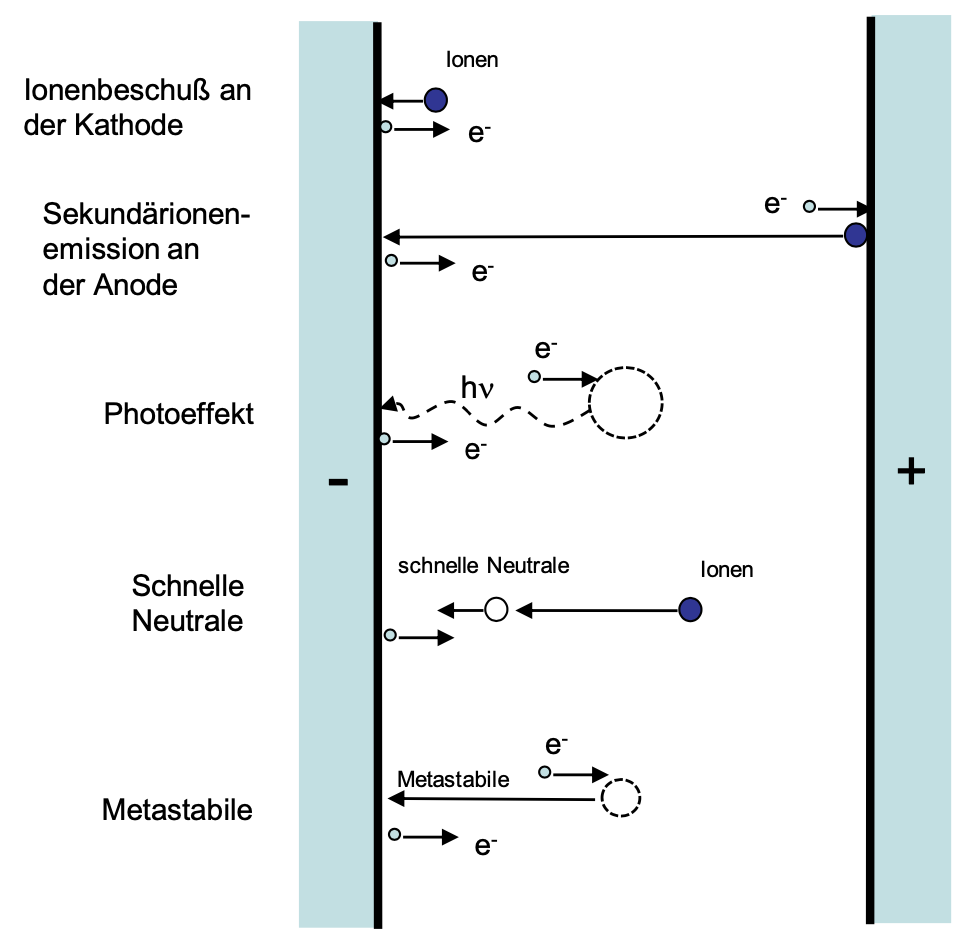
\includegraphics[width=0.7\linewidth]{bilder/see}
	\caption{Die verschiedenen Mechanismen der Sekundärelektronenemission. Bild aus \cite{keudellVorlesungsskriptEinfuhrungPlasmaphysik2010}.}
	\label{fig:see}
\end{figure}

Ionen sind aber nicht der einzige Mechanismus der SEE. Besonders angeregte metastabile Gasteilchen sind in niedrig ionisierten Plasmen in deutlich höherer Konzentration vorhanden als Ionen. In Simulationen eines He-Mikroplasmas zeigte sich eine Dichte metastabiler Heliumteilchen von \qtyrange{2e14}{3e14}{cm^{-3}}, die mehr als zwei Größenordnungen über der Dichte der Heliumionen liegt \cite{kothnurStructureDirectcurrentMicrodischarge2003}. Diese geben beim Kontakt mit der Anode durch ihre Abregung genug Energie ab, um Elektronen zu emittieren. Besonders in Atmosphärendruckplasmen geben Ionen ihren Impuls wegen der hohen Gasdichte zudem oft über Stöße an neutrale Gasteilchen ab, welche beim Aufprall auch Elektronen aus der Kathode stoßen können. Sekundärelektronen können außerdem durch Lichtteilchen im photoelektrischen Effekt herausgelöst werden. Da der Fluss neutraler Teilchen nicht durch elektrische Methoden messbar ist, wird die Anzahl aller SE trotzdem im Verhältnis zur Anzahl der Ionen angegeben. In diesem \textit{effektiven SEE Koeffizienten} (ESEEC) $ \gamma_E $ werden also auch andere Emissionsmechanismen betrachtet. In der Praxis ergeben sich für diesen Werte von etwa $ 0,\!3 $ bei Niederdruck \cite{arumugamEffectiveSecondaryElectron2017} und etwa 1 bei Normaldruck \cite{hansenConventionalNonconventionalDiagnostics2022}. Dabei ist der ESEEC sowohl vom Material, als auch insbesondere von der Struktur der Oberfläche abhängig \cite{phelpsColdcathodeDischargesBreakdown1999}.


Da z.B. die Elektronen herauslösenden Neutralteilchen zuvor durch Stöße mit Ionen beschleunigt wurden, welche schlussendlich auch auf die Kathode treffen, ist der Anteil anderer Mechanismen an der SEE grob proportional zum Ionenstrom. Dies macht die Angabe des ESEEC sinnvoll, da dieser unabhängig von der Größe des Ionenstroms ist. Da im ESEEC auch Sekundärelektronen berücksichtigt werden, die nicht durch Ionen erzeugt wurden, ist dieser zwangsweise größer als der Koeffizient $ \gamma_I $. Zudem ist der ESEEC druckabhängig und bei Normaldruck deutlich höher als bei Niederdruck \cite{phelpsColdcathodeDischargesBreakdown1999}.

\subsection{Messung der ESEEC}

Zur Bestimmung der effektiven SEE Koeffizienten wird die thermische Leistung auf der Kathode mit der elektrischen Leistung am Plasma verglichen. Der elektrische Strom $ I $ durch die Kathode setzt sich aus zwei Teilen zusammen: Dem Ionenstrom $ I_\text{i,C} $ durch das Auftreffen positiver Ionen auf das Substrat und dem Elektronenstrom $ I_\text{se,C} $ durch das Ablösen von Elektronen aus der Oberfläche \cite{liebermanPrinciplesPlasmaDischarges2005,chapmanGlowDischargeProcesses1980a,phelpsColdcathodeDischargesBreakdown1999}
\begin{align*}
	I = I_{\text{se,C}} + I_{\text{i,C}}.
\end{align*}
Diese beiden Anteile stehen durch den ESEEC in Relation, da dieser die Anzahl emittierter Elektronen pro Ion angibt \cite{arumugamEffectiveSecondaryElectron2017}. Es gilt $ I_{\text{se,C}} = \gamma_E I_{\text{i,C}}$ und damit
\begin{align*}
	I = I_{\text{i,C}} (1+\gamma_\text{E}).
\end{align*}
Da die Ionen von der anliegenden Spannung beschleunigt werden, ist die von den Ionen aufgenommene Leistung gleich dem Produkt aus Ionenstrom und Spannung \cite{kerstenEnergyBalanceSubstrate2001, arumugamEffectiveSecondaryElectron2017}:
\begin{align*}
	U \cdot I &= U\cdot I_{\text{i,C}}(1+\gamma_\text{E})\\ 
	P_{\text{el}} &= P_\text{i} \cdot (1+\gamma_\text{E})
\end{align*}

Auch wenn nicht alle Leistung auf die Kathode von Ionen abgegeben wird, wird sie doch zunächst von Ionen aus dem elektrischen Feld aufgenommen. Die Energie, die z.B. ein durch Stöße mit Ionen beschleunigtes Neutralteilchen an die Kathode abgibt, sorgt dafür, dass ebendiese Ionen entsprechend weniger Energie zur Kathode führen. Überdies werden die Ionen vor allem in der Randschicht direkt vor der Kathode beschleunigt, sodass die durch Stöße beschleunigten Neutralteilchen vorrangig die Kathode erhitzen. Im Netto ist deshalb die thermische Leistung an der Kathode gleich der Leistung an den Ionen durch die anliegende Spannung \cite{sheridanCollisionalPlasmaSheath1991,arumugamEffectiveSecondaryElectron2017,trottenbergMeasurementForceExerted2015a}:
\begin{align*}
	P_\text{therm,C} = P_\text{i}
\end{align*}
Damit kann der ESEEC durch
\begin{align*}
	\gamma_\text{E} = \dfrac{P_\text{el}}{P_\text{therm,C}} -1 
\end{align*}
aus den gemessenen Daten berechnet werden. Die auf diese Methode erlangten Werte sind vorsichtig zu interpretieren, da in den vereinfachten Annahmen z.B. nicht auf Energieverluste, die nicht auf die Sonden treffen, oder die Kinetik der Teilchen \cite{phelpsColdcathodeDischargesBreakdown1999, phelpsUseSecondaryelectronYields1999} eingegangen wird. Trotzdem eignen sie sich um Trends, zum Beispiel gegenüber den Werten bei Niederdruck oder den Ionen-SEE-Koeffizienten, zu betrachten.

\section{Optische Emissionsspektroskopie}

Die optische Emissionspektroskopie (OES) ist eine verbreitete Methode der Plasmadiagnostik, mit der man die Zusammensetzung des Plasmas bestimmen kann. Dabei wird die optische Strahlung des Plasmas im Spektroskop mit einem Brechungsgitter in die verschiedenen Wellenlängen aufgeteilt. In dem so gemessenen Spektrum zeigen sich Emissionslinien, die dadurch entstehen, dass die elektronisch angeregten Atome im Plasma bei ihrer Abregung um ein bestimmtes Energieniveau Strahlung einer charakteristischen Wellenlänge abgeben:
\begin{align*}
	h\nu = \dfrac{hc}{\lambda} = \Delta E
\end{align*}

Da die möglichen Differenzen der Energieniveaus von Element zu Element verschieden sind, lässt sich aus dem Ort der Emissionslinien im Spektrum bestimmen, welche Elemente im Plasma vorhanden sind. In dieser Arbeit wird so überprüft, ob eine reine Gasatmosphäre hergestellt werden konnte, oder ob Verunreinigungen durch andere Gase im Spektrum erkennbar sind.